\section{Introduction and Open Loop
Discussion}\label{introduction-and-open-loop-discussion}

\begin{wrapfigure}{r}{0.45\textwidth}
  \begin{center}
  \vspace{-20pt}
  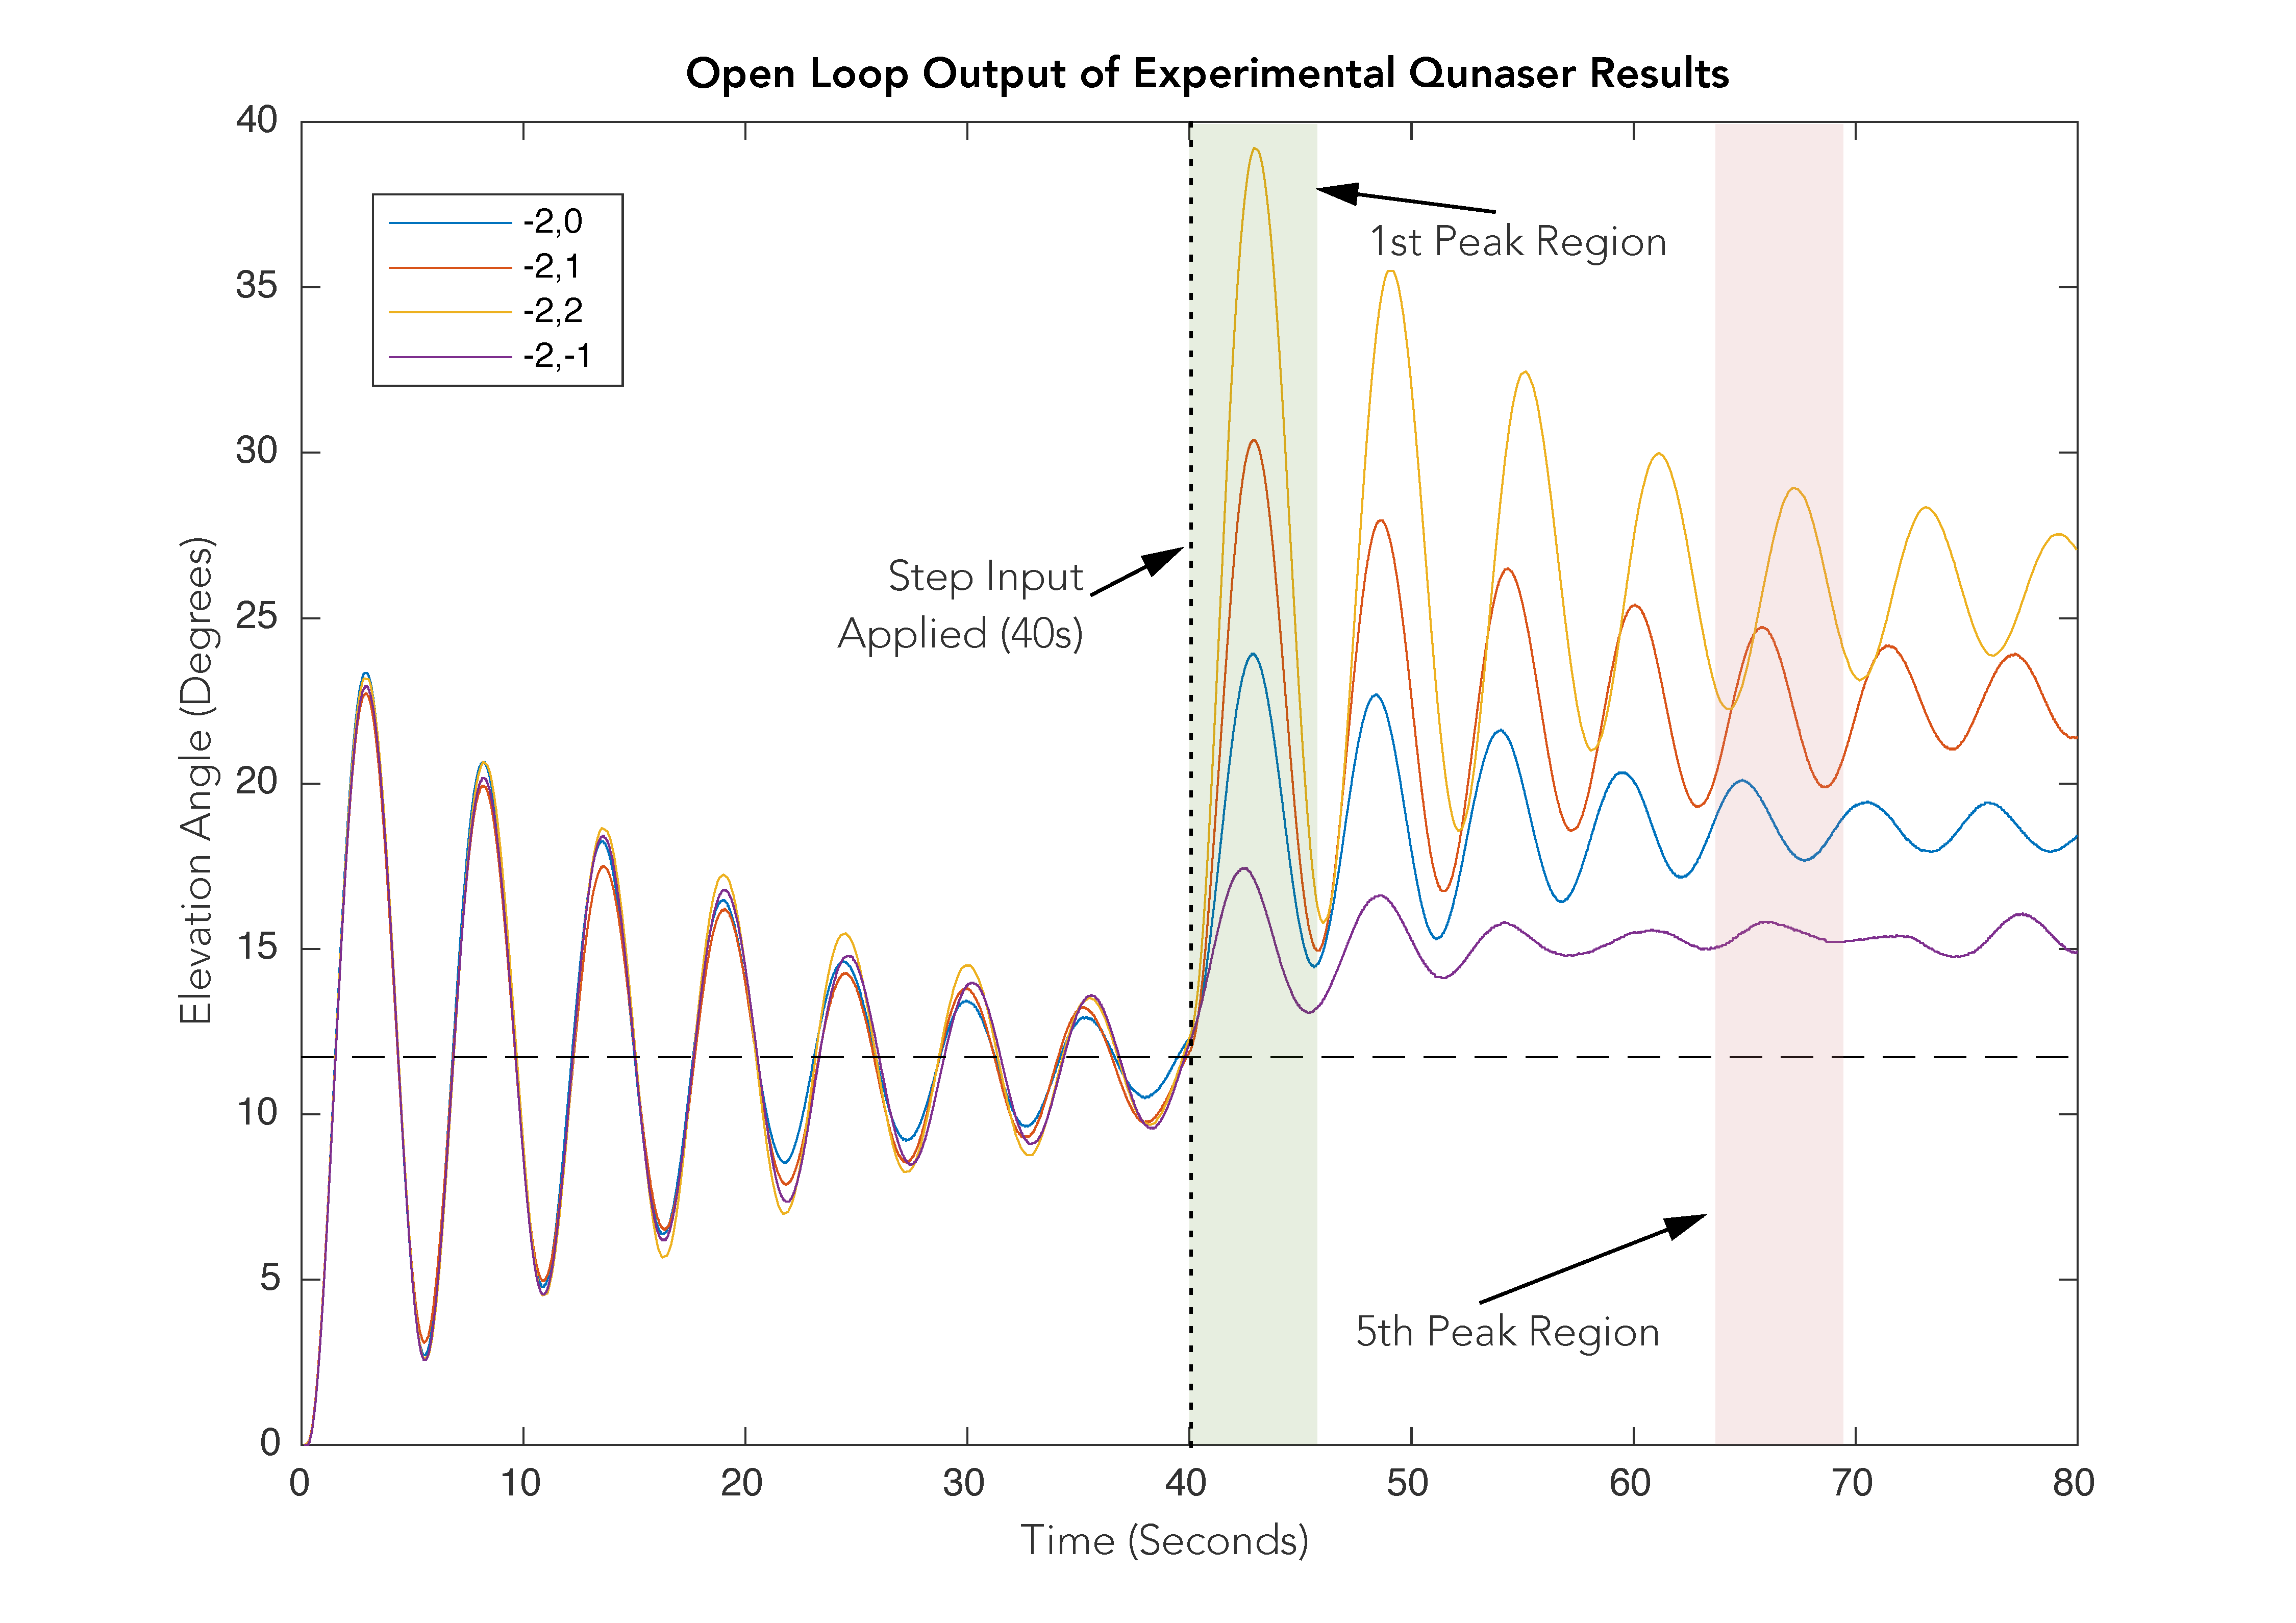
\includegraphics[trim = 50 20 50 10, clip, width=0.44\textwidth]{intrograph.pdf}
  \end{center}
  \caption{Graph Showing the Open Loop Nature of the Experimental Quanser Response}
  \label{intrograph}
  \vspace{-15pt}
\end{wrapfigure}

This report compares the experimental and theoretical transfer functions
of 3 degree of freedom Quanser-Control rig. Control design is important
to understand the behaviour of a dynamic system, and then improve the
performance. Sensors and actuators are used in the Quanser to measure
and vary performance characteristics of the Quanser. In this case, an
elevation change was introduced to the Quanser in order to observe an
oscillating damped behaviour. Measuring this response a theoretical
transfer function was then estimated.

An Open-Loop system is a where behavioural characteristics can be
controlled manually. These changes are not feedback into the system,
therefore the output has no effect on the input of the system
\cite{openloop} meaning self-correction is not possible. In the case of
the Quanser-Control Rig, elevation angle was independent of the output
and manually controlled, whereas pitch and travel data was manually
feedback to the system. Figure \ref{intrograph} shows the open loop
behaviour of the elevation axis, as the elevation angle was varied
between 10 and 40 degrees.

\section{Method and Results}\label{method-and-results}

\begin{wrapfigure}{r}{0.45\textwidth}
  \vspace{0pt}
\captionof{table}{Table Showing Key Parameter Calculations \cite{vibnote},\cite{vibnote2}}
  \begin{center}
  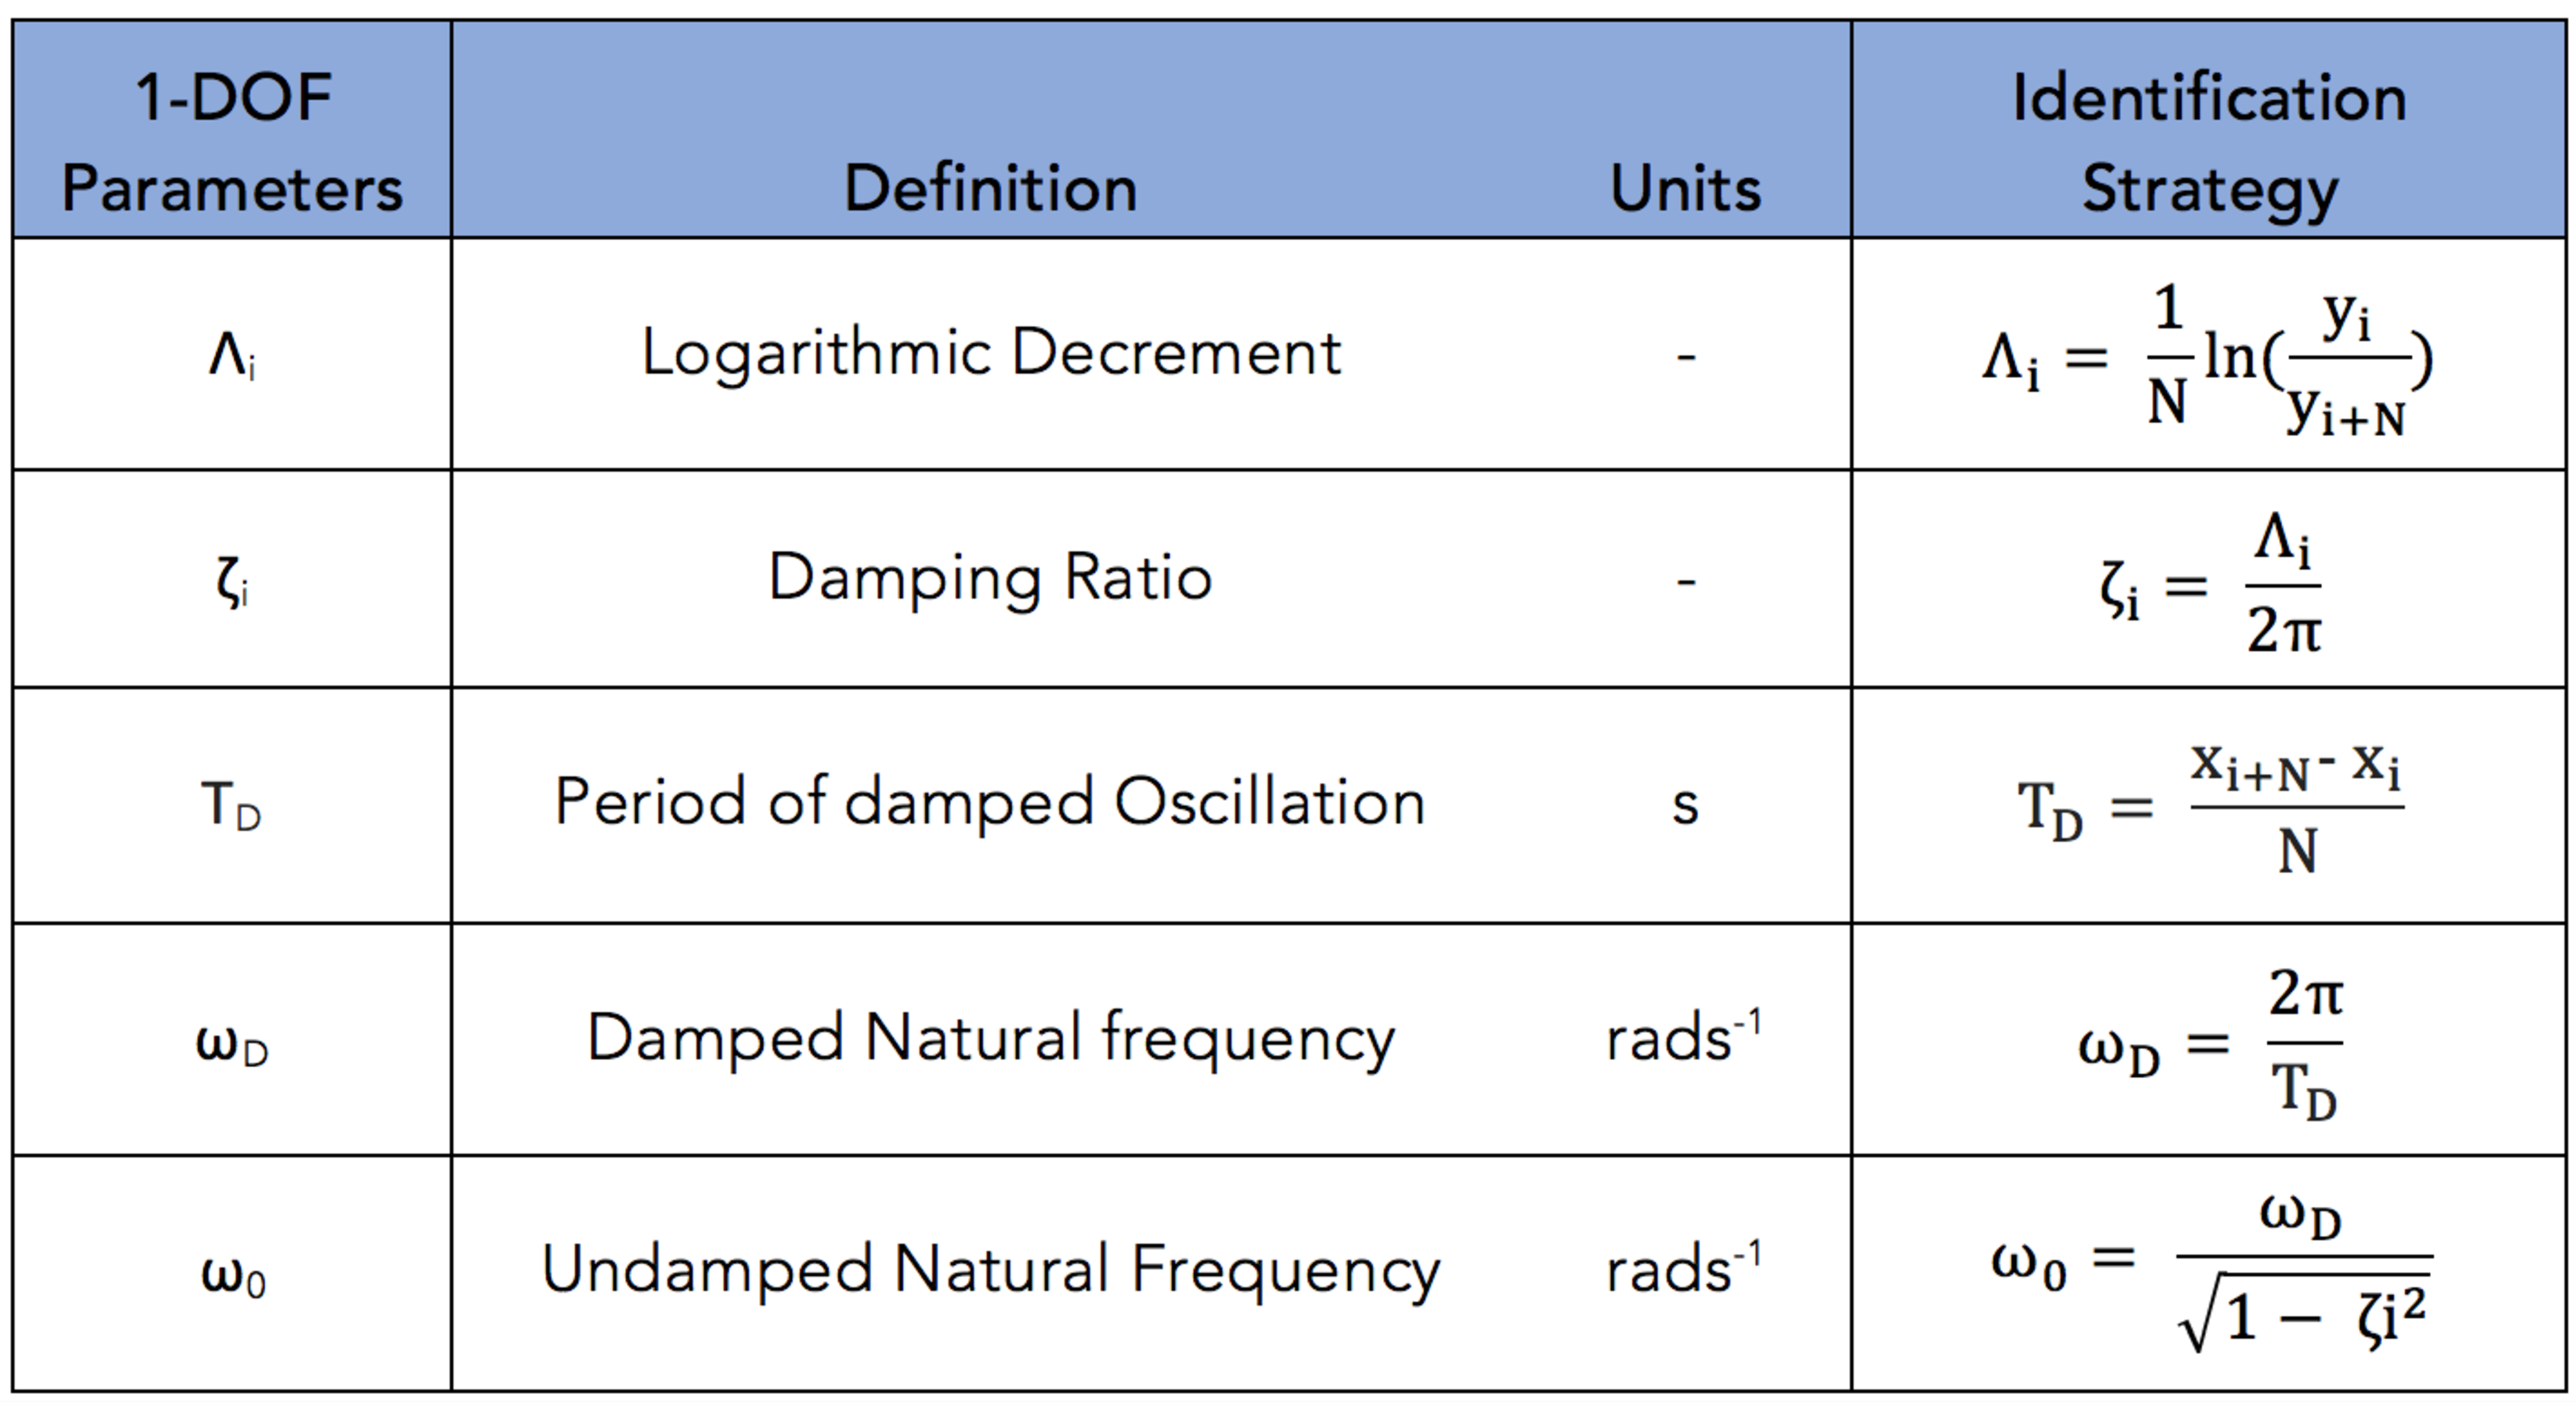
\includegraphics[trim = 0 0 0 0, clip, width=0.4\textwidth]{eqtable.pdf}
\end{center}
\label{eqtable}
  \vspace{0pt}
\end{wrapfigure}

\subsection{Finding Experimentation Results from
Quansers}\label{finding-experimentation-results-from-quansers}

\begin{enumerate}

\item
  Replace the elevator input with a step block, using the parameters:
  Start Time: 40s, Start Value: -2, End Value: -1 to 2. This was used to
  automate the step input at a specific time for each elevator input
  test. A step input time of 40s was chosen to allow the initial
  response to settle to an acceptable level (see Figure
  \ref{intrograph}).
\item
  Use range of elevator input values, varying from an initial value of
  -2 to 2 in steps of 1. Repeat each test case, saving workspace
  variables.
\item
  Check data for anomalies, Averaged repeats for valid results across
  the different step inputs.
\end{enumerate}

\subsection{Analyse Transfer Function}\label{analyse-transfer-function}

\begin{enumerate}

\item
  Isolate elevation values for corresponding inputs from 40s to 80s;
  this captures this captures the response after step input.
\item
  In order to estimate a transfer function - the following parameters
  were calculated: Natural frequency, Undamped natural frequency and
  damping ratio, refer to Table \ref{eqtable}.
\end{enumerate}

\subsubsection{Second Order}\label{second-order}

To calculate the Second Order Transfer-Function, a forced response
behaviour was noted. Using Table \ref{eqtable} equations \cite{vibnote}
\cite{vibnote2}, in addition to the x and y values taken from the peaks
highlighted in figure \ref{intrograph} the logarithmic decrement and the
period of damp oscillation was approximated. Using these equations
values for the damping ratio \(\zeta\) and natural frequency
\(\omega_n\) were obtained and substituted into the formal equation
shown in equation \ref{2otf}.

\begin{align}
\frac{ y(s) }{ u(s) } &=\frac{ k\cdot \omega_{ n }^{ 2 } }{ s^{ 2 }+2\zeta \omega_{ n }s+\omega_{ n }^{ 2 } }
\label{2otsf}
\end{align}

In order to obtain a single transfer function which represents the
system as a whole for varying elevators angle steps, estimated transfer
functions were found for each test case. These parameters were then
averaged obtaining a single fit transfer function where gain was changed
to model different elevator angle step inputs. This captured some of the
behaviour of the system as step level varied.

\begin{wrapfigure}{r}{0.5\textwidth}
  \begin{center}
  \vspace{0pt}
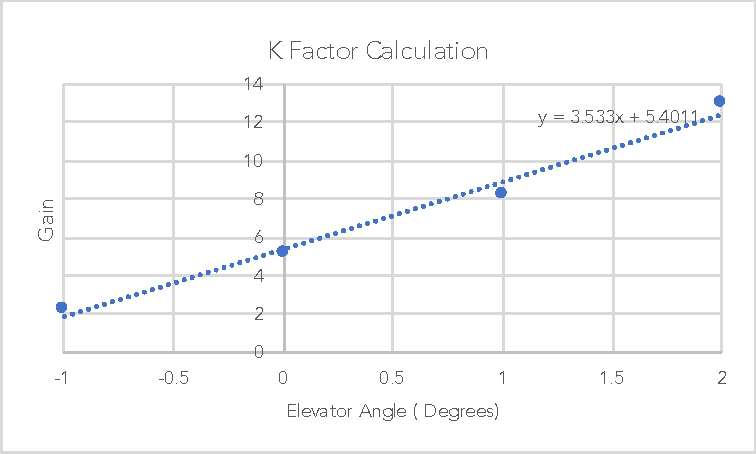
\includegraphics[trim = 10 10 10 10, clip, width=0.49\textwidth]{kgraph.pdf}  
\end{center}
\caption{Graph Finding the Gain For Each Step Input}
\label{kgraph}
  \vspace{0pt}
\end{wrapfigure}

To calculated the a representative gain scaling factor \(k\) for each of
the step inputs, max elevation for each step input was taken (from the
first peak shown in Figure \ref{intrograph}). These values were plotted
on a graph to find their correlation, shown in figure \ref{kgraph}. The
gain \(k\) value was heuristically adjusting to match the estimated
amplitude with the experimental results from -2 to 2, where it was found
that \(k = 0.26\). This value was used to translate the correlation
equation between points into scaling factors.

After applying this method, amplitudes for all the steps fitted more
closely. Finally damping ratio and undamped natural frequency were
tweaked to give the final fit, again by trial and error.

\subsubsection{First Order}\label{first-order}

Standard First Order Response Transfer Function:

\begin{align}
 \frac { y(s) }{ u(s) } &=\frac { k }{ \tau s+1 }
\label{fos}
\end{align}

Due to the Quanser-Control Rig being a Second Order System Equation
\ref{fos} was not applicable for finding the First Order Transfer
Function. Instead this was estimated by considering the Second Order
Transfer Function case where: \(\zeta =1\) and \(s^2=0\).

\begin{align}
\frac { k\cdot \omega_{ n }^{ 2 } }{ 2\zeta \omega_{ n }s+\omega_{ n }^{ 2 } } &\rightarrow \frac { k\cdot \omega_{ n }^{ 2 } }{ 2\omega_{ n }s+\omega_{ n }^{ 2 } }
\end{align}

\section{Results}\label{results}

\begin{align}
&\text{2nd Order Transfer Function}: && k \cdot \frac { 1.109 }{ s^{ 2 }+0.1313s+1.109 }
\end{align}

\begin{align*}
\\
&\text{Where:} &&\zeta = 0.0623 &&& \omega_n = 1.0532
\\
\end{align*}

\begin{align}
&\text{1st Order Transfer Function}: && k \cdot \frac { 1.109 }{ 2.106s+1.109 }
\end{align}

\begin{align*}
\\
&\text{Where:} &&\zeta = 1 &&& \omega_n = 1.0532
\\
\end{align*}

\begin{figure}[H]
\centering
\begin{minipage}{.49\textwidth}
\centering
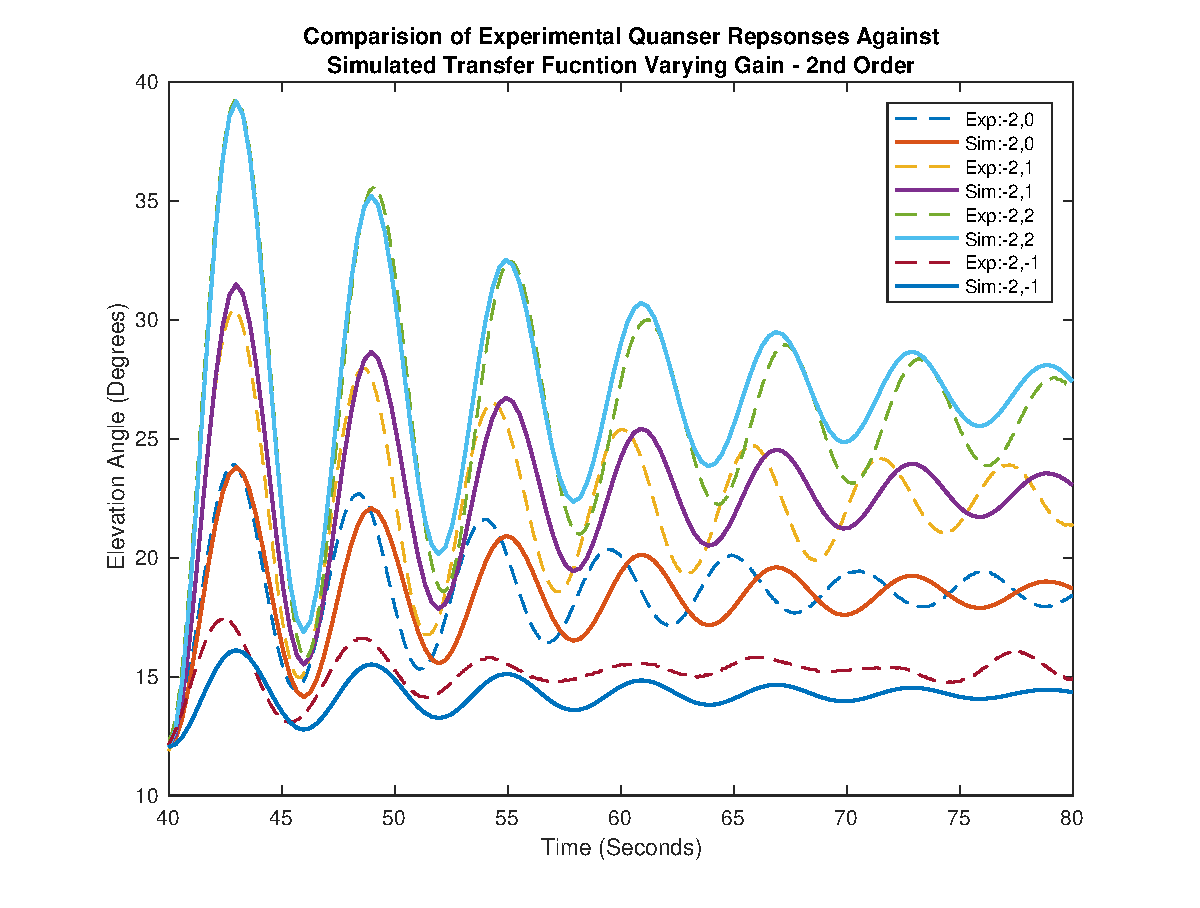
\includegraphics[trim = 35 16 35 0, clip, width=0.995\textwidth]{2ndTFcomp.eps}
\caption{2nd Order Simualted Transfer Function Comparision}
\label{2ndTFcomp}
\end{minipage}
\hfill
\begin{minipage}{.49\textwidth}
  \centering
  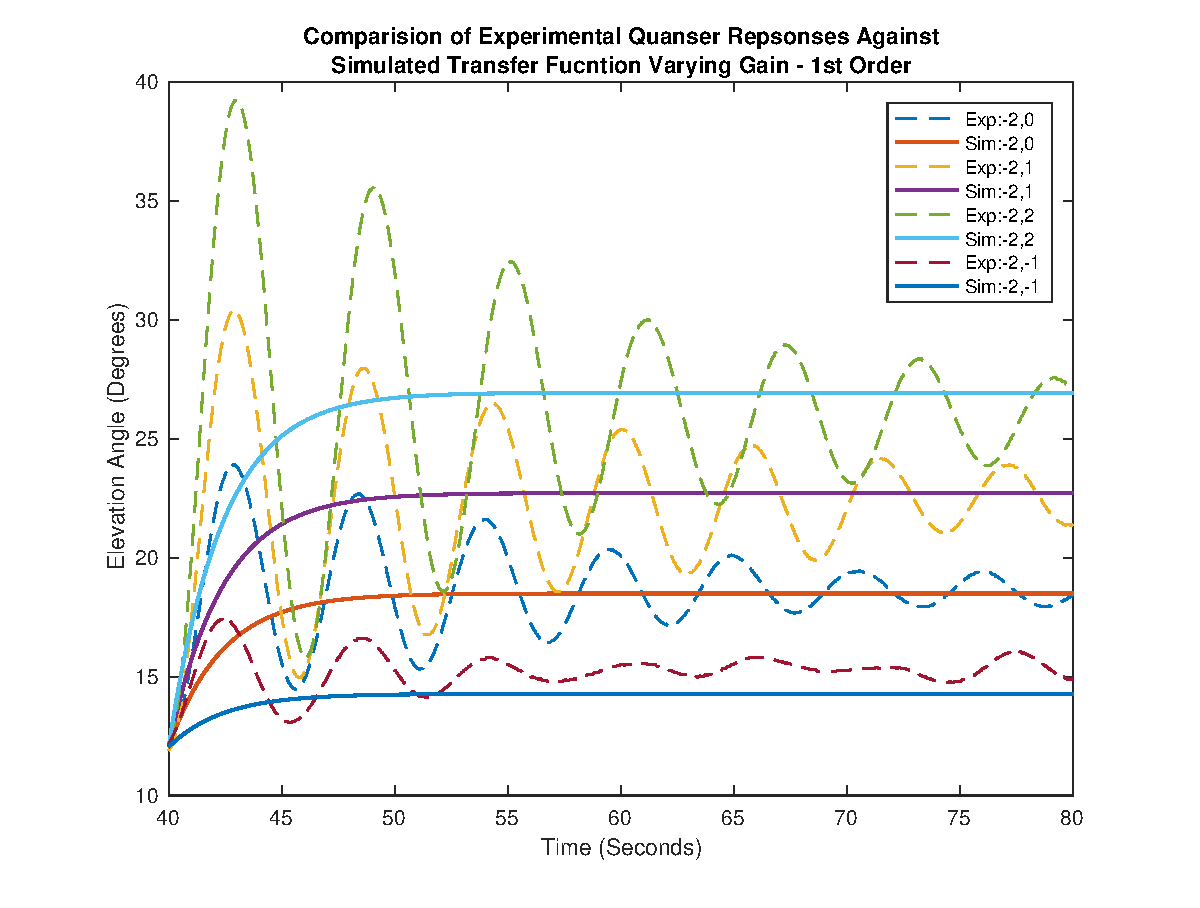
\includegraphics[trim = 35 16 35 0, clip, width=0.995\textwidth]{1stTFcomp.eps}
  \caption{1st Order Simualted Transfer Function Comparision}
  \label{1stTFcomp}
\end{minipage}
\end{figure}

\section{Observations and Analysis:}\label{observations-and-analysis}

Experimental elevator input

\begin{itemize}
\tightlist
\item
  Step input of 2 was used as the datum which the scaling factors of the
  other steps was matched against. This results in the 2 step graph
  being a better fit than the others
\item
  There is an observable phase and amplitude deviation
\item
  Peak amplitude prediction becomes worse for lower amplitude cases
\item
  The upper experimental oscillations were slightly larger than the
  lower oscillations
\end{itemize}

\begin{wrapfigure}{r}{0.45\textwidth}
  \begin{center}
  \vspace{0pt}
  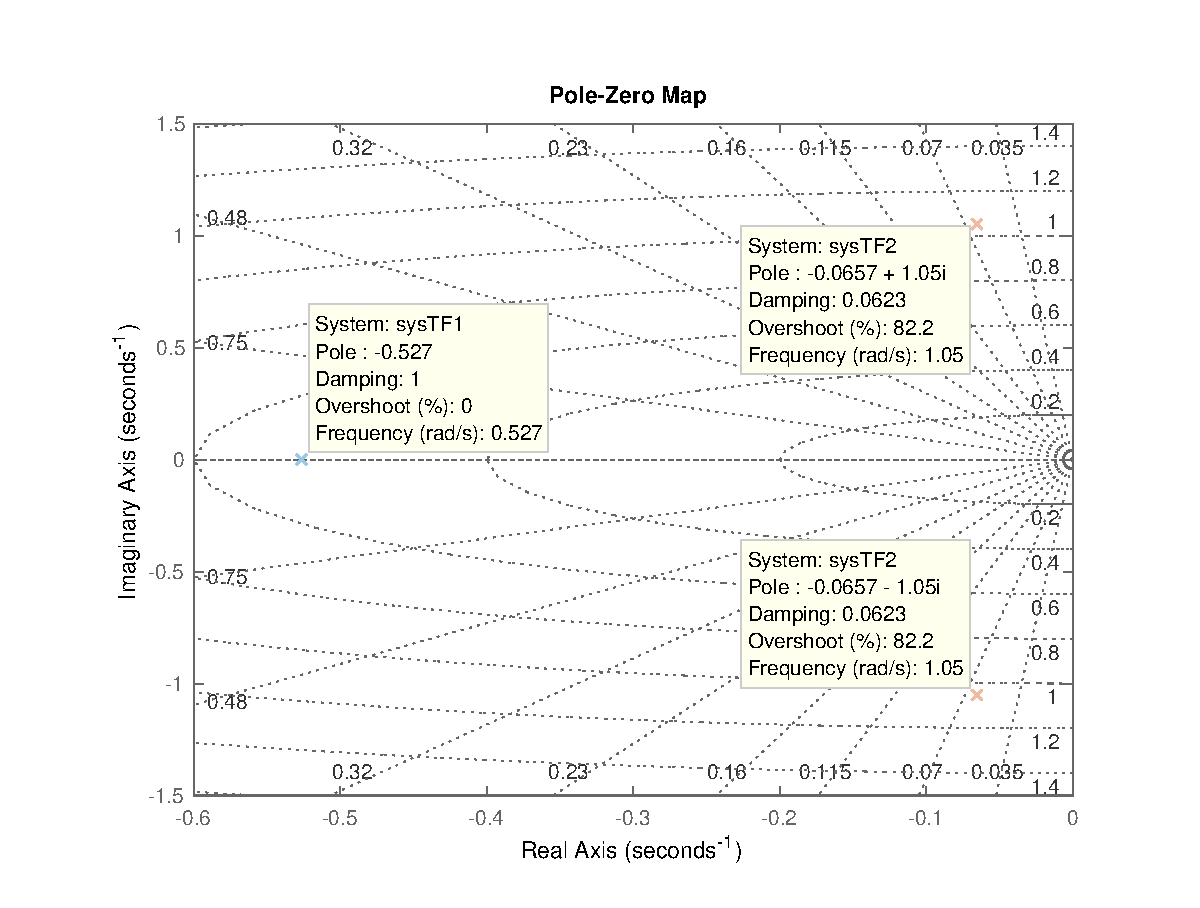
\includegraphics[trim = 35 14 35 0, clip, width=0.5\textwidth]{poleszmap.eps}
  \end{center}
  \caption{Map of the Poles}
 \label{poleszmap}
  \vspace{-25pt}
\end{wrapfigure}

Root Locus plot

\begin{itemize}
\tightlist
\item
  The grid lines represent lines of constant damping and lines of
  natural frequency
\item
  Second order transfer function root locus has a pair of points with an
  imaginary axis component (complex root) - This shows the underdamped
  nature of the system as 0\textless{}zeta\textless{}1
\item
  First order transfer function Root locus point exists purely in the
  real axis component.
\item
  Increase in gain for the second order shows these roots becoming more
  positive and negative in the imaginary axis respectively
\item
  Increase in gain for the first order shows the root becoming more
  negative along the real axis
\end{itemize}

\subsection{Potential Errors}\label{potential-errors}

During the quanser operation, a significant observable error was the
drift in the quanser-- this was more noticeable when during longer runs.
This is potentially due to accumulating error increasing with time
duration. Whilst the Quansers have error correcting features -- this is
only sensitive to a finite degree so could be considered imperfect. This
implies errors may accumulate for a greater run time as the system fails
to accurately correct for inconsistencies. Another source of deviation
from MATLAB's theoretical transfer function step response - could be the
inaccuracy in step input time. Whilst a step block was introduced in the
simulink model to automate the `elevator input' at 40 seconds - upon
closer observation of the response plots, this was not the case. This
was potentially due to accumulated lag in the system and the controller
- as a result of computational latency. As a result this likely
influenced the initial condition - causing a phase and amplitude shift
in experimental results. Another effect of this is; the introduction of
error in logarithmic decrement and period of damped frequency
calculation as peak points were potentially taken from `error' shifted
values. In theory the step input is modelled as an immediate action -
whilst experimentally the step response acted over time - this adds to
the error shift of the values.

Physically when the Quanser was in operation, there were physical
factors to consider when exploring the errors. Friction in the Quanser
support hinge potentially resulted in a slightly decreased elevation
than desired - this adds to the natural damping response of the system
and may explain why the experimental curves in Figure(?) are more
compacted time wise than the MATLAB transfer function step plot. However
it is useful to note that the MATLAB transfer function was estimated by
averaging test cases and hence is derived empirically. The slightly
decreased elevation is also compounded by physical wires in the rig
which acted as a small `jamming' mechanism to the system.

As with any control system, noise can be introduced by external and
internal factors. In the Quanser system - gyro noise and wind resistance
were major factors. Sensors in any system measure quantities which need
to be controlled - in this case the elevator sensor sampling was stored
values at discrete points. Whilst the sampling time was quite small so
captured the general nature of the oscillating damped curves - some
critical points may have been missed due to this for example at the
point of highest amplitude, the inflexion behaviour begins after a
region of constant amplitude. Theoretically we see a quicker inflexion
transition in this region. see Figure ()?.

Due to the instruction of never taking a step from the `fans off'
position (as there are high nonlinear effects during startup) - the
initial elevator input was set to -2 (to get the fans running) and then
after 40 seconds a elevator step was input into the system. For this
reason the step input may have been applied during mid oscillation past
the steady state elevation position - this likely either amplified or
decreased the actual step input depending on which stage of oscillation
the quanser is at.
